% Thesis Presentation
% compile using PDFTeXify or PDFLaTeX
\documentclass[11pt,compress]{beamer}

\mode<presentation> {
\setbeamertemplate{blocks}[rounded][shadow=true]
%\usetheme{Madrid}
%\usetheme{Warsaw}
\usetheme{Montpellier}
\usecolortheme{rose}  % color theme
\setbeamertemplate{theorems}[numbered]
%\setbeamercovered{transparent}
%\usefonttheme[onlymath]{serif}
\usefonttheme{serif}
%\usetheme{boxes}
\setbeamertemplate{navigation symbols}{}
\setbeamertemplate{itemize items}[circle]  % ball, circle
\setbeamertemplate{enumerate items}[square]

\setbeamertemplate{footline}{%
  \hfill%
  \usebeamercolor[fg]{page number in head/foot}%
  \usebeamerfont{page number in head/foot}%
  \insertframenumber \,/\,\inserttotalframenumber
  \kern1em\vskip2pt%
}

}

\setbeamertemplate{headline}{	% navigation bar of section (second headline)
\begin{beamercolorbox}{section in head/foot}
   \vskip2pt\insertnavigation{\paperwidth}\vskip2pt
\end{beamercolorbox}
\begin{beamercolorbox}[colsep=1.5pt,ht=.3ex]{upper separation line head}  % separator [colsep=1.5pt,ht=.3ex]
\end{beamercolorbox}
}

\makeatletter
\let\beamer@writeslidentry@miniframeson=\beamer@writeslidentry%
\def\beamer@writeslidentry@miniframesoff{%
  \expandafter\beamer@ifempty\expandafter{\beamer@framestartpage}{}% does not happen normally
  {%else
    % removed \addtocontents commands
    \clearpage\beamer@notesactions%
  }
}
\newcommand*{\miniframeson}{\let\beamer@writeslidentry=\beamer@writeslidentry@miniframeson}
\newcommand*{\miniframesoff}{\let\beamer@writeslidentry=\beamer@writeslidentry@miniframesoff}
\makeatother


%--------- 宏包  ----------
\usepackage[UTF8,noindent]{ctex}
\usepackage[english]{babel} %show english numerate
\usepackage{epsfig,amssymb,amsmath,version}
\usepackage{amssymb,version,graphicx,fancybox,mathrsfs,multirow}
\usepackage{booktabs}
\usepackage{epstopdf}
\usepackage{url,hyperref}
\usepackage{tabularx,array,makecell}
\usepackage{color,xcolor}
\usepackage{cases}
\usepackage{mathtools}
%\usepackage{zhlipsum}

%----------- 定义行距 ---------------
\renewcommand{\baselinestretch}{1.15}

% 定义新表格命令
\newcolumntype{P}[1]{>{\centering \arraybackslash}p{#1}}
\newcolumntype{L}{>{\quad}X}
\newcolumntype{C}{>{\centering \arraybackslash}X}
\newcolumntype{R}{>{\raggedright \arraybackslash}X}


%---------- 设置中文字体  ---------------
\setbeamerfont{normal text}{family=\kaishu}
\setbeamerfont{frametitle}{family=\kaishu}
\setbeamerfont{title}{family=\kaishu}
\setbeamerfont{subtitle}{family=\kaishu}
\setbeamerfont{institute}{family=\kaishu}
\setbeamerfont{author}{family=\kaishu}
\setbeamerfont{headline}{size=\heiti}
\setbeamerfont{footline}{family=\kaishu}
\setbeamerfont{section in toc}{family=\kaishu}
\setbeamerfont{subsection in toc}{family=\kaishu}

%---------- 定理设置  --------------
\setbeamertemplate{theorems}[numbered]
\newtheorem{thm}{Theorem}
\numberwithin{thm}{section}
\newtheorem{defn}{Definition}
\numberwithin{defn}{section}
\newtheorem{lmm}{Lemma}
\numberwithin{lmm}{section}
\newtheorem{pro}{Proof}
\theoremstyle{example}
\newtheorem{exam}{Example}
%\numberwithin{exam}{section}

\setbeamertemplate{caption}[numbered]
\numberwithin{figure}{section}
\numberwithin{table}{section}
\numberwithin{equation}{section}

\makeatletter
\newcommand\HUGE{\@setfontsize\Huge{36}{42}}
\makeatother

% 定义文字颜色
\newcommand{\red}[1]{\textcolor{red}{#1}}
\newcommand{\blue}[1]{\textcolor{blue}{#1}}


%\AtBeginSection[]
%{ \begin{frame}
%    \frametitle{Outline}
%    \tableofcontents[currentsection,hideallsubsections] %currentsubsection
%  \end{frame}
%  \addtocounter{framenumber}{-1}  %目录页不计算页码
%}


%----------------------------------------------------------------------------------------
%	TITLE PAGE
%----------------------------------------------------------------------------------------

\title[论文题目]{毕业论文题目毕业论文题目毕业论文题目}

\author[学生姓名]
{
  报告人:学生姓名~~~ \vskip 3mm
  专业:专业名称 \vskip 3mm
  指导教师:导师姓名 ~ 职称 \vskip 3mm
  研究方向:专业研究方向
}

\institute[学校名称]{}
%\institute[学校名称]{\normalsize 学校名称}

\date[2020.x.x]{2020.x.x}

\graphicspath{{./Figures/}}

\begin{document}
\songti

{\setbeamertemplate{headline}{}
\begin{frame}
\titlepage % Print the title page as the first slide
\end{frame}}

\begin{frame}
\frametitle{Outline}
\tableofcontents
\end{frame}

%----------------------------------------------------------------------------------------
%	PRESENTATION SLIDES
%----------------------------------------------------------------------------------------

%------------------------------------------------
\section{文本与 Block}
%------------------------------------------------

\begin{frame}{文本测试}
这是一段测试文字。这是一段测试文字。这是一段测试文字。这是一段测试文字。这是一段测试文字。这是一段测试文字。
这是一段测试文字。这是一段测试文字。这是一段测试文字。这是一段测试文字。这是一段测试文字。这是一段测试文字。

\vspace{1ex}
这是一段测试文字。这是一段测试文字。这是一段测试文字。这是一段测试文字。这是一段测试文字。这是一段测试文字。
这是一段测试文字。这是一段测试文字。这是一段测试文字。这是一段测试文字。这是一段测试文字。这是一段测试文字。

\end{frame}

%-----------------------------------------------

\begin{frame}
\frametitle{Blocks of Highlighted Text}
\begin{block}{Block 1}
Lorem ipsum dolor sit amet, consectetur adipiscing elit. Integer lectus nisl, ultricies in feugiat rutrum, porttitor sit amet augue.
\end{block}

\begin{exampleblock}{Block 2}
Pellentesque sed tellus purus. Class aptent taciti sociosqu ad litora torquent per conubia nostra, per inceptos himenaeos.
\end{exampleblock}

\begin{alertblock}{Block 3}
Suspendisse tincidunt sagittis gravida. Curabitur condimentum, enim sed venenatis rutrum, ipsum neque consectetur orci, sed blandit justo nisi ac lacus.
\end{alertblock}
\end{frame}

%------------------------------------------------
\section{列表环境}

\begin{frame}
\frametitle{Bullet Points}
\begin{itemize}[<+-| alert@+>]
\item Lorem ipsum dolor sit amet, consectetur adipiscing elit
\item Aliquam blandit faucibus nisi, sit amet dapibus enim tempus eu
\item Nulla commodo, erat quis gravida posuere, elit lacus lobortis est, quis porttitor odio mauris at libero
\item Nam cursus est eget velit posuere pellentesque
\item Vestibulum faucibus velit a augue condimentum quis convallis nulla gravida
\end{itemize}
\end{frame}

%------------------------------------------------

\begin{frame}
\frametitle{Multiple Columns}
\begin{columns}[c] % The "c" option specifies centered vertical alignment while the "t" option is used for top vertical alignment

\column{.45\textwidth} % Left column and width
\textbf{Heading}
\begin{enumerate}
\item Statement
\item Explanation
\item Example
\end{enumerate}

\column{.5\textwidth} % Right column and width
Lorem ipsum dolor sit amet, consectetur adipiscing elit. Integer lectus nisl, ultricies in feugiat rutrum, porttitor sit amet augue. Aliquam ut tortor mauris. Sed volutpat ante purus, quis accumsan dolor.

\end{columns}
\end{frame}

%------------------------------------------------
\section{表格与定理}
%------------------------------------------------

\begin{frame}
\frametitle{表格和引理}
\begin{table}
\caption{Table caption}
\begin{tabular}{l l l}
\toprule
\textbf{Treatments} & \textbf{Response 1} & \textbf{Response 2}\\
\midrule
Treatment 1 & 0.0003262 & 0.562 \\
Treatment 2 & 0.0015681 & 0.910 \\
Treatment 3 & 0.0009271 & 0.296 \\
\bottomrule
\end{tabular}
\end{table}
\begin{lmm} \upshape
  For any $v \in H_{A}^{r}(\Lambda)$ and $r \geq 0$,
  \begin{equation}
    \|P_{N} v-v\| \leq c N^{-r}\|v\|_{r, A}.
  \end{equation}
\end{lmm}
\end{frame}

%------------------------------------------------


\begin{frame}
\frametitle{定理}

\begin{thm}[Lax-Milgram Lemma] \upshape
Let $X$ be a Hilbert space, let $a(\cdot, \cdot)$ : $X \times X \rightarrow \mathbb{R}$ be a continuous and coercive bilinear form, and let $F : X \rightarrow \mathbb{R}$ be a linear functional in $X^{\prime}$. Then the variational problem:
\begin{equation}
  \alert{
  \left\{\begin{aligned}
  &\text {Find } u \in X \text { such that } \\
  &a(u, v)=F(v), \forall v \in X
  \end{aligned} \right. }
\end{equation}
has a unique solution. Moreover, we have

\begin{equation}
  \alert{ \|u\| \leq \frac{1}{\alpha}\|F\|_{X^{\prime}}  }
\end{equation}
\end{thm}

\end{frame}

%------------------------------------------------

\begin{frame}[fragile] % Need to use the fragile option when verbatim is used in the slide
\frametitle{Verbatim}
\begin{exam}[Theorem Slide Code]
\begin{verbatim}
\begin{frame}
\frametitle{Theorem}
\begin{theorem}[Mass--energy equivalence]
$E = mc^2$
\end{theorem}
\end{frame}\end{verbatim}
\end{exam}

\begin{thm}[Mass--energy] \upshape
$E = mc^2$
\end{thm}

\end{frame}


\begin{frame}
\frametitle{论文进度安排}
\begin{table}[htp!]
\centering
\renewcommand\arraystretch{1.3} %定义表格高度
% PLCR前面已经定义
\begin{tabularx}{0.92\textwidth}{|P{3.2cm}|C|}
\Xhline{2\arrayrulewidth}
论文起止时间       &  论文筹备过程\\
\hline
2019.xx -- 2019.xx    &  论文定题,整理相关文献\\
\hline
2020.xx -- 2020.xx    &  审查、修改、完成开题报告\\
\hline
2020.xx -- 2020.xx   &  对论文排版、初步完成论文初稿\\
\hline
2020.xx -- 2020.xx    &  毕业论文预答辩\\
\hline
2021.xx -- 2021.xx    &  对论文进行补充、完善\\
\hline
2021.xx -- 2021.xx    &  论文定稿\\
\hline
2021.xx -- 2021.xx    &  毕业论文答辩\\
\Xhline{2\arrayrulewidth}
\end{tabularx}
\end{table}

\end{frame}


%------------------------------------------------

\section{插图环境}

\begin{frame}
\frametitle{Figure}

Uncomment the code on this slide to include your own image from the same directory as the template .TeX file.
\begin{figure}[htp!]
\centering
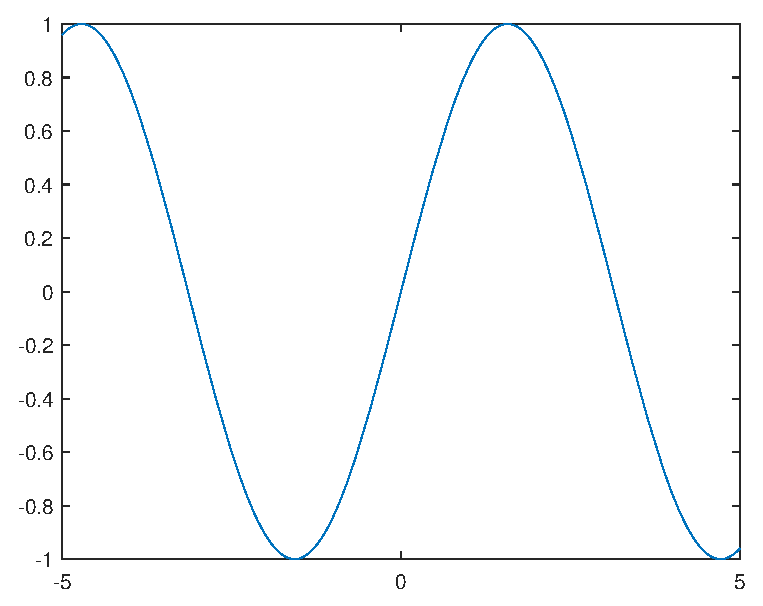
\includegraphics[width=0.5\linewidth]{image1}
\caption{Caption of Figure 1.} \label{fig:A}
\end{figure}
\end{frame}

%------------------------------------------------

\begin{frame}
\frametitle{Figure 2}
\begin{figure}[htb]
\centering
\begin{minipage}{0.48\linewidth}
\centering
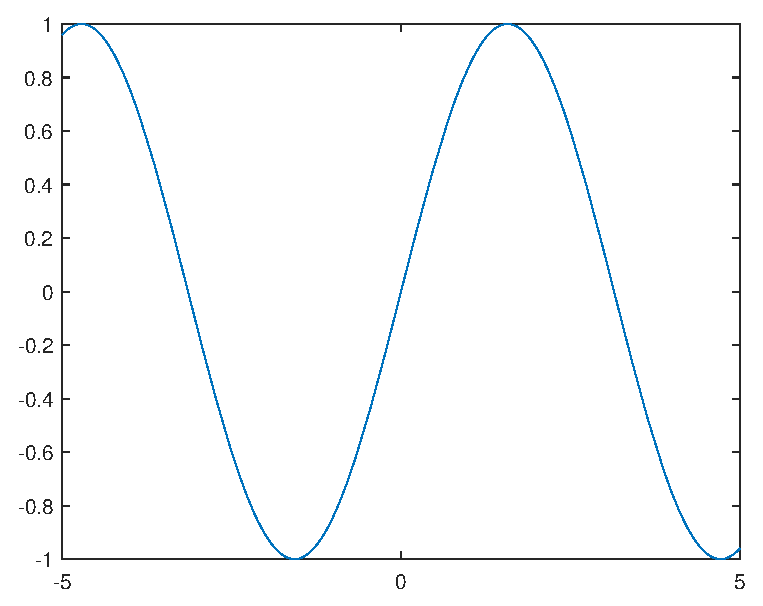
\includegraphics[width=\linewidth]{image1}
\caption{Caption of Figure 1.}
\end{minipage}\hfill
\begin{minipage}{0.48\linewidth}
\centering
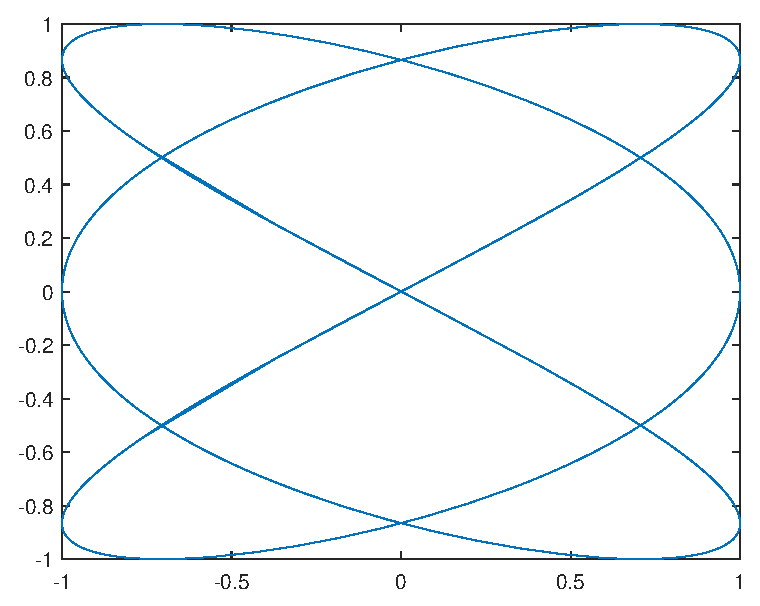
\includegraphics[width=\linewidth]{image2}
\caption{Caption of Figure 2.}
\end{minipage}
\end{figure}
\end{frame}


%------------------------------------------------
\section{参考文献}
%------------------------------------------------

\begin{frame}[fragile] % Need to use the fragile option when verbatim is used in the slide
\frametitle{Citation}
An example of the \verb|\cite| command to cite within the presentation:\\~

This statement requires citation \cite{p1}.
\end{frame}

%------------------------------------------------

\begin{frame}
\frametitle{References}
\footnotesize{
\begin{thebibliography}{99} % Beamer does not support BibTeX so references must be inserted manually as below
\bibitem[Smith, 2012]{p1} John Smith (2012), Title of the publication, \emph{Journal Name} 12(3), 45 -- 678.
\end{thebibliography}
}
\end{frame}


%------------------------------------------------

% get rid of navigation bars in beamer
\miniframesoff

%\setbeamertemplate{background canvas}[vertical shading][bottom=white,top=structure.fg!25]
\setbeamertemplate{headline}{}
\begin{frame}
\sffamily
\begin{center}
\HUGE{\textcolor[RGB]{165,3,3}{Thank~you!}}
\end{center}
\end{frame}

%----------------------------------------------------------------------------------------

\end{document}
